\section{Discussion}
\label{chap:Discussion}

\subsection{Data processing}
\label{chap:Data processing}

\quad This project's first step was to load the data and split it between a training set and a validation set. Since there are a few more necessary preprocessing steps before the classifier can be trained, this split is taken care of in the \texttt{BOW} class, found in \texttt{preprocessing.py}.
This split must be done before counting word occurrences to ensure the counter has not seen any of the data used to tune the model. 
Another critical aspect of the splitting is to ensure the distribution between the labels is preserved in both sets.

\begin{figure}[!h]
\centering
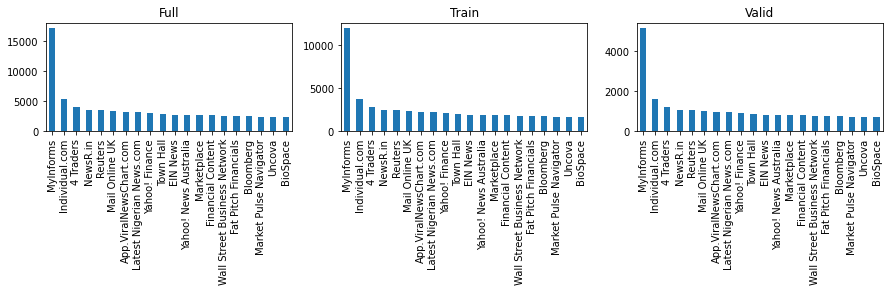
\includegraphics[width=1\linewidth]{pictures/source_dist.png}
\caption{Source distributions}
\end{figure}

This distribution was maintained by using the \texttt{sklearn.utils.resample} method and providing the source column for the \texttt{stratify} parameter. The ratio between entries in the training set and validation set was set to 0.7, in the \texttt{train\_size} parameter when initializing a \texttt{BOW} class object. 

The \texttt{resample} method returns a subset of size \texttt{n\_samples} of the original data, as long as the \texttt{resample} parameter is set to false. The number of samples was found multiplying the provided proportion with the length of the original data. The output from \texttt{resample} was stored as the training set. 

The validation set was then found by pulling all the remaining data points from the original data set, by filtering on the indexes \textit{not} in the train set. A code snippet of this process is shown below.

\begin{minted}{python}
n = len(df) * train_prop

train = sklearn.utils.resample(
    df,
    replace=False,
    stratify=df.source,
    n_samples=n
)

test = df[~df.index.isin(train.index)]
{python}\end{minted}

\subsection{Training a classifier}
\label{chap:Training a classifier}

\quad A precise formulation of the task at hand can be as follows:

\begin{quote}
    Given a list of words in a document, \textbf{predict the source} of the document. 
\end{quote} 

The algorithm needed to define a common vocabulary for the input data and convert the documents into bag-of-words vectors to later feed into the classifier. 

A b.o.w. transformation converts raw text documents to count vectors, disregarding grammar, stop words, and any other irrelevant characters. The counts that replaced each word correspond to the number of times that word is found in the training set, as long as it is part of the common vocabulary. Note that since the original data was split into a training and validation set, word occurrences in the \textit{validation} set are \textit{not} included in this counting. 
\newline
Specifically, the assignment asked to test three different types of bag-of-words techniques for this representation. The chosen types for this project were:

\begin{itemize}
\item \texttt{counter} These b.o.w. vectors are the actual counts of that word in the common vocabulary.

\item \texttt{binary}: Instead of the numeric counts, a word is represented as a binary value, depicting whether or not that word is a part of the common vocabulary.

\item \texttt{tfidf}: Like the \texttt{counter} representation, this b.o.w. vector type replaces the word with a numeric value. The difference here is that the word counts are normalized according to how many other documents this same word occurs. The idea is to weed out ubiquitous words that are not predefined as stop words. 
\end{itemize}

The size of the common vocabulary was determined by a tunable hyper-parameter \texttt{vocab\_size}, which is taken in as a parameter for new \href{https://github.uio.no/fabior/IN5550/blob/master/Oblig1/packages/preprocessing.py}{\texttt{BOW}} instances. The definition of this parameter already in the initialization of \href{https://github.uio.no/fabior/IN5550/blob/master/Oblig1/packages/preprocessing.py}{\texttt{BOW}} objects allowed for hard definitions of tensor shapes, avoiding expensive and unnecessary computations. More on this parameter in the \hyperref[sec:tuning]{feature tuning section}. 

Before actually training and tuning the classifier, the last step was to extract the gold source labels for the input data. These are the true labels for each data point, and are found in the attribute \texttt{y\_train} for \href{https://github.uio.no/fabior/IN5550/blob/master/Oblig1/packages/preprocessing.py}{\texttt{BOW}} objects.\\

Discussion around the model's parameters along the model's best performance can be found in the upcoming sections.

\subsection{Feature tuning}
\label{sec:tuning}
\label{chap:tuning}

\quad Table \ref{table:default_params} shows the initial default values chosen for the classifier:



\begin{table}[H]
    \centering
    \begin{tabular}{ |c|c|c|c|c| }
        \hline
        \multicolumn{5}{|c|}{\textbf{Hyper-parameters}} \\
        \hline
        \textbf{Hidden Layers} & \textbf{Units} & \textbf{Epoch} & \textbf{Mini-batch} & \textbf{Dropout} \\
        \hline
        1 & 25 & 20 & 32 & 0.2 \\
        \hline
         \textbf{Bias} & \textbf{Learning Rate} & \textbf{Momentum} & \textbf{Loss-Function}& \\
        \hline
        0.1 & 0.01 & 0.9 & Cross-Entropy &\\
        \hline
    \end{tabular}
    \caption{Initial model parameters}
    \label{table:default_params}
\end{table}

The values for these initial parameters were not entirely random. Arguments for the choice of default values are given below:

\begin{itemize}
    \item \texttt{Bias}, \texttt{learning rate} and \texttt{momentum} were set as their default value.
    \item \texttt{Batch size} was initialized to 32 as per instructed.
    \item \texttt{Loss-function} was initialized to cross-entropy because it is typically used for multi-label classifications.
    \item \texttt{Hidden layers} was initialized to 1 to make the simplest initial model.
    \item \texttt{Epochs} was initialized to 20 after trying out several different epochs and seeing no improvement after about 20.
    \item \texttt{Units}
    \item \texttt{Dropout} was initialized to 0.2 after seeing a lot of variance without regularization.
\end{itemize}

Tuning the classifier was done semi-automatically with the help of the \href{https://github.uio.no/fabior/IN5550/blob/master/Oblig1/packages/studies.py}{\texttt{packages/studies.py}} file. This module consists of multiple different \texttt{Study} classes for each of the different parameter pairs this group decided to test. The encapsulation of the classes helped maintain efficient memory usage and made for straightforward and understandable tuning. 

An \href{https://github.uio.no/fabior/IN5550/blob/master/Oblig1/packages/evaluation.py}{\texttt{packages/evaluation.py}} script created executed the studies for each of the tuning steps. It was this file that generated the results presented below. These results are stored in the \href{https://github.uio.no/fabior/IN5550/blob/master/Oblig1/output}{\texttt{output}} directory. 

The plots were produced using the \href{https://github.uio.no/fabior/IN5550/blob/master/Oblig1/plot.py}{\texttt{plot.py}} script, along with the header of the file to plot as a command-line argument.


\subsubsection{Activation functions}
\quad The first parameters tuned were the activation functions, both in the hidden-layers and in the output-layer. Four different activation functions were tested for each of these, giving a total of 16 possible combinations. These were \texttt{["sigmoid", "tanh", "relu", "softmax"]}. 

The metrics used to decide which combinations of activation functions were optimal for each position were the times, accuracy, and F1 scores of each model. As shown in Figure \ref{fig:act_heatmap}, the best candidate gave the lowest possible time and highest possible accuracy and F1-score. 

Here, it is essential to note that the F1-score is a more reliable metric than the accuracy since the distribution between classes was not entirely balanced. While accuracy measures the percentage of correct classifications, the F1-score gives a measurement of the combination of precision (number of correctly classified over the total number of samples) and recall (number of correctly classified over the total number that should have been classified with that label). For this task, a macro F1-score was needed since there were multiple labels to classify. The formula for calculating a macro F1 score is given below, where $N$ represents the number of classified labels.

$$
\text{Macro }F_1 = \frac{1}{N} \sum_{i=0}^{N} \frac{\text{precision}_i\cdot\text{recall}_i}{\text{precision}_i+\text{recall}_i}
$$


\begin{figure}[H]
\centering
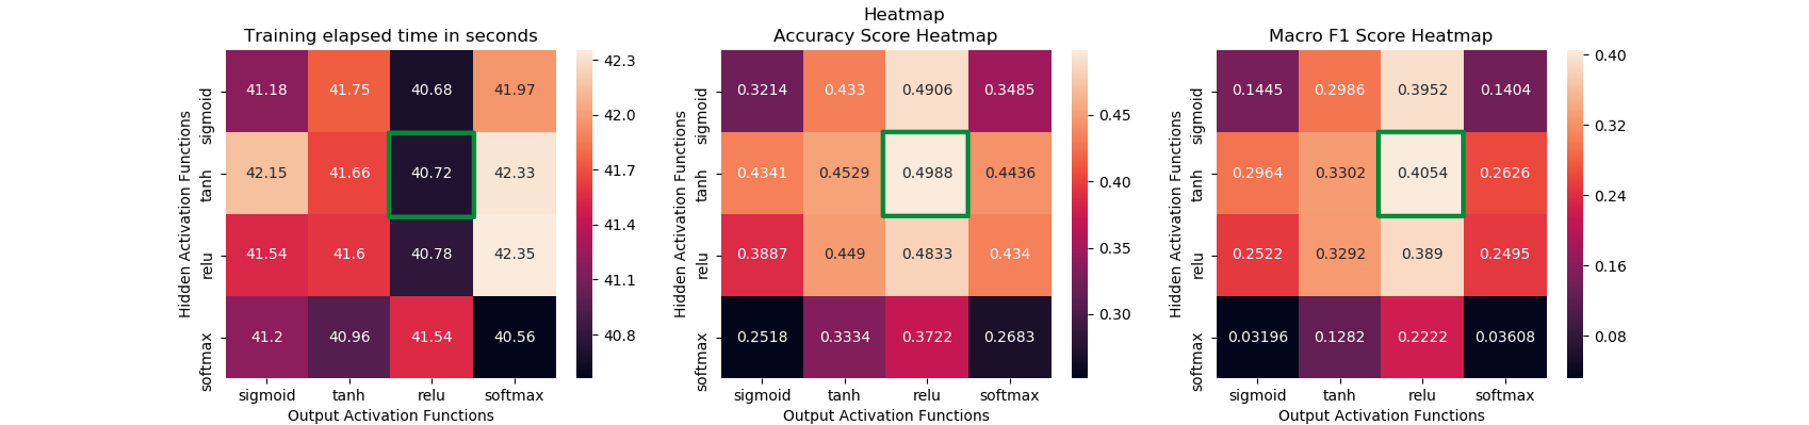
\includegraphics[width=1\linewidth]{pictures/activation_heatmap.png}
\caption{Heat maps for activation function tuning}
\label{fig:act_heatmap}
\end{figure}

The optimal combination of activation functions was the hyperbolic tangent on the hidden layers, with relu on the output layer. This decision was reasonably straight-forward since for each of the heat maps shown in Figure \ref{fig:act_heatmap}, this combination gave the best score according to the criterion previously mentioned. \\

\subsubsection{Bag of Words Type and Vocabulary Size}
\quad The second set of parameters tuned was the vocabulary sizes and the b.o.w types. We tested a range of $\in[50, 30000]$ as vocabulary sizes and three variations of b.o.w: \texttt{binary}, \texttt{tfidf}, and \texttt{counter}. These were performed using the function \texttt{BOWStudy} in \href{https://github.uio.no/fabior/IN5550/blob/master/Oblig1/packages/studies.py}{\texttt{packages/studies.py}}.

As with tuning the activation functions, the metrics in focus when tuning the optimal bag-of-words parameters were times, accuracy, and F1-scores for each model. The training time is increasing linearly with the size of the input vectors after vocab\_size

$\approx 5000$

As displayed in \ref{fig:bow_heatmap} the best candidate is the values that yielded the best F1-score and accuracy compared to the training time. 

\begin{figure}[H]
\centering
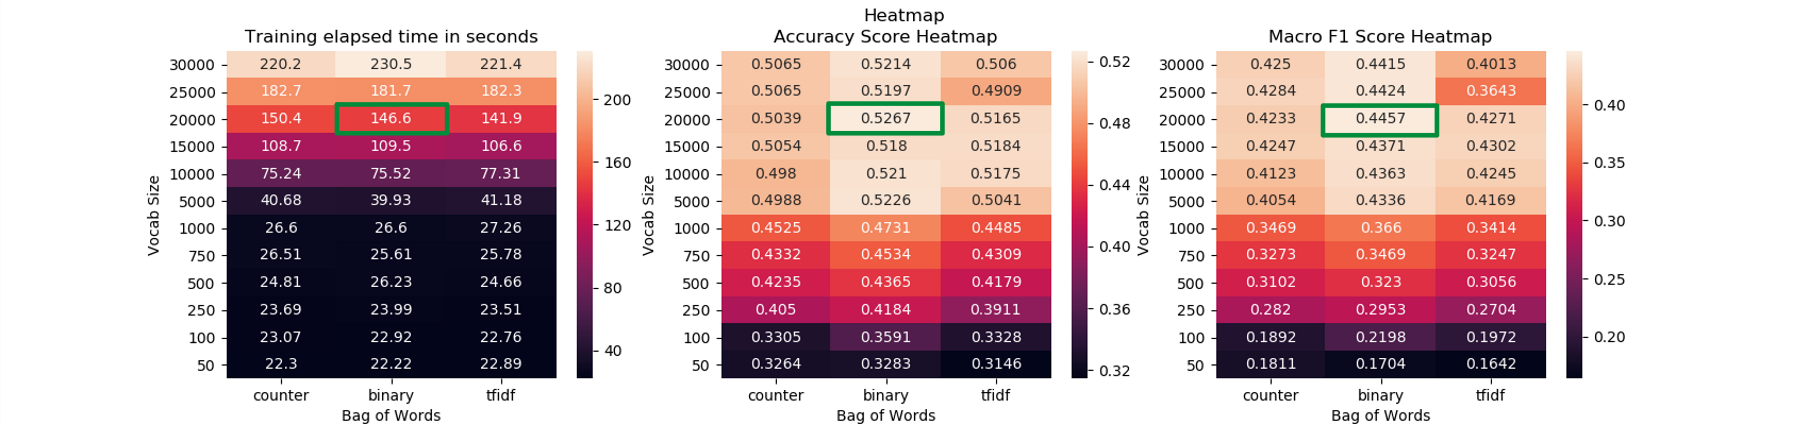
\includegraphics[width=1\linewidth]{pictures/bow_heatmap.png}
\caption{Heat maps for vocabulary sizes and bag-of-words types.}
\label{fig:bow_heatmap}
\end{figure}

Looking at \ref{fig:bow_heatmap} it is pretty clear that the optimal settings found from this study were a vocabulary size of 20000 with the binary counter for the CountVectorizer as this setting yielded the best accuracy \textit{and} F1-scores while still training reasonably fast compared to the larger vocabulary sizes.

\subsubsection{Part of Speech (PoS) analysis}

\quad One typical technique applied in NLP for feature tuning is POS (Part of speech), which considers the types of the words and how much information these groups can bring for training the artificial neuron network models. We filtered the entire vocabulary for capturing a specific given word type, or combination of that, per time and then performed the model's training and evaluation as follows:

\begin{table}[H]
\centering
\begin{tabular}{ |p{6.5cm}||p{2cm}|p{2cm}|  }
\hline
\multicolumn{3}{|c|}{Part of Speech (PoS) Analysis}\\
\hline
Vocabulary & Acc. score & F1-score\\
\hline
all PoS together                &   0.5267  &   0.4457\\
only VERB                       &   0.3938  &   0.2966\\
only ADJ                        &   0.3700  &   0.2819\\
only PROPN                      &   0.4057  &   0.3290\\
only NOUN                       &   0.4420  &   0.3568\\
only ADV                        &   0.3316  &   0.2123\\
NOUN and PROPN                  &   0.4820  &   0.4026\\
NOUN and PROPN and VERB         &   0.5110  &   0.4319\\
NOUN and PROPN and VERB and ADJ &   0.5032  &   0.4265\\
NOUN and PROPN and VERB and NUM &   0.5131  &   0.4298\\
\hline
\end{tabular}
\caption{Results with the most common 20.000 words and Binary Bag of Words (BoW) type for a given PoS vocabulary.}
\label{table:Standard_Parameters}
\end{table}

It is important to mention that the word type \texttt{NOUN} had the highest individual score, showing that this category brings more relevant information than the others. However, as shown in Table \ref{table:Standard_Parameters}, the best PoS combination is still the vocabulary containing the most common 20.000 words for all PoS together. 

\subsection{Measuring time efficiency}
\label{chap:Measuring time efficiency}

\subsubsection{Epochs and Batch Size}
\quad The next step after finding the ideal shape of input vectors was to find approximately how many epochs were necessary for training the neural network. This step was decided to be done here to save time and avoid the hassle of training unnecessary epochs for the remaining optimization. The fewer epochs needed, the faster future models could be built, meaning more efficient parameter tuning.

The batch size was tested together with epochs since they are used to measure time efficiency. A range of $\in[32, 60]$ was checked here, along with an outlying $500$ as a control.

Again, heat maps were used to help visualize these statistics:

\begin{figure}[H]
\centering
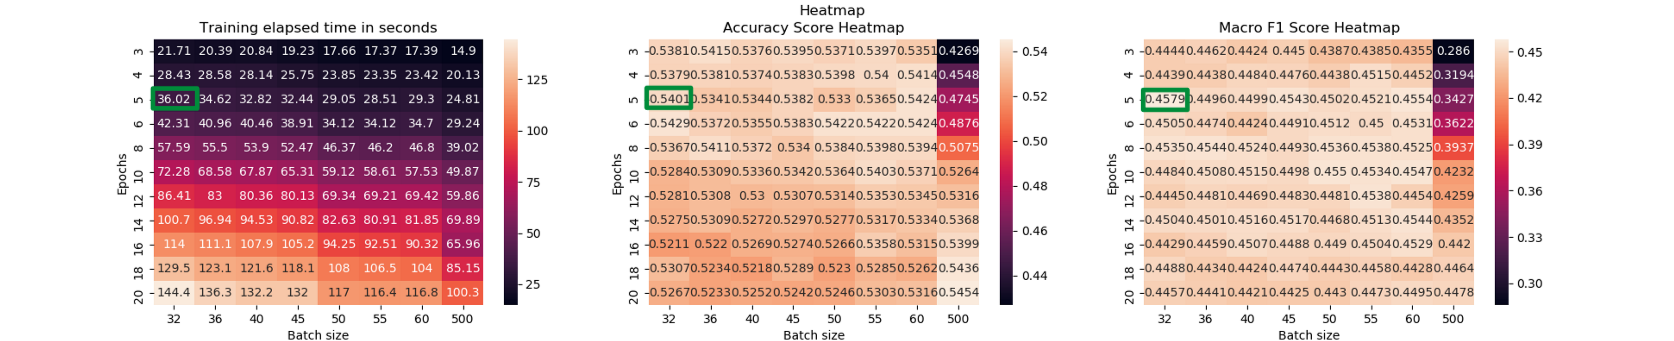
\includegraphics[width=1\linewidth]{epoch_heatmap}
\caption{Heat maps for epoch and batch size optimization}
\label{fig:epoch_heatmap}
\end{figure}

It was found that the model converged quickly, giving good enough scores already after only five epochs. The smaller batch sizes were preferred over more extensive, although the variation between (most of) the batch sizes analyzed in this step proved to be relatively small. The control size of $500$ was used to help highlight that smaller sizes were preferred. 

After these results and deductions, we decided to stick with five epochs and a batch size of 32 for all future models.

\subsubsection{Hidden Layers and Units per Layer}
\quad After most of the heavy and computationally expensive parameters were tuned, it was time to optimize the number of hidden layers. The number of units per layer was decided as an excellent match to optimize with this parameter since they both deal with the network's inner architecture.

Given that the assignment specifically asked to test at least five different numbers of hidden-layers, the group decided to test hidden-layer values in the range $\in[1, 6]$. For the number of units, the range of $\in[10, 2000]$ was decided to encompass as many candidates as possible. The capability to check up to 2000 units highlights how beneficial it was to tune epochs \textit{before} hidden layers. Especially taking into account that the time exploded as the values for each parameter combo grew, as seen in Figure \ref{fig:hlu_heatmap}.

\begin{figure}[H]
\centering
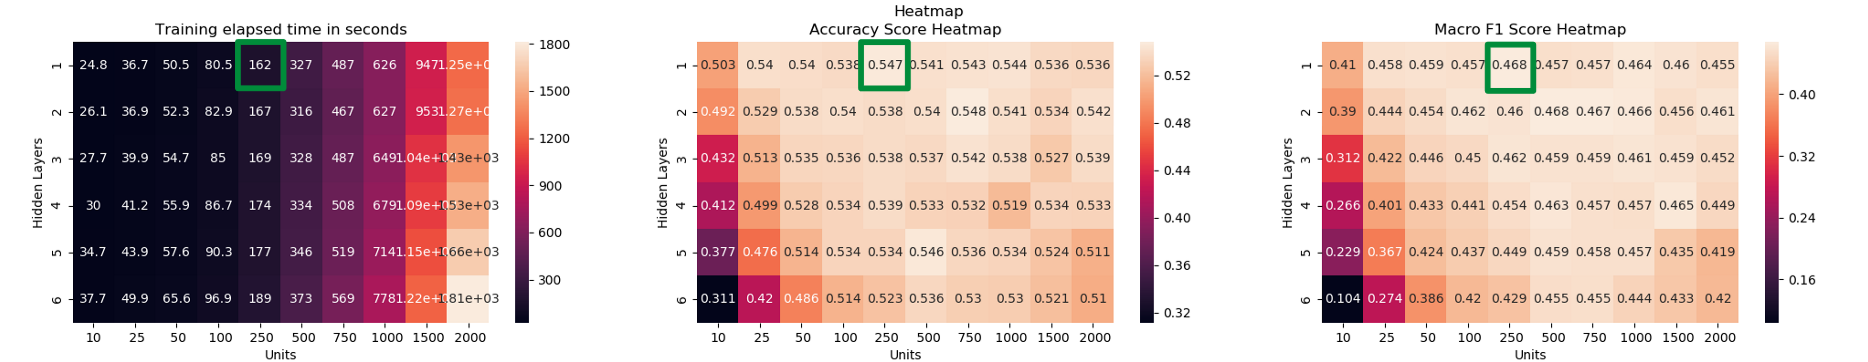
\includegraphics[width=1\linewidth]{hiddenlayer_heatmap}
\caption{Heat maps for number of hidden layer and units optimization}
\label{fig:hlu_heatmap}
\end{figure}

Surprisingly enough, the F1-score and accuracies did not vary much as the number of hidden layers increased. Instead, it looks as if the best accuracy was achieved already with only 1-2 hidden layers. As expected, computation time increased almost linearly with the number of units. This increase occurred because more units per hidden-layer mean more computations both in forward and backward propagation. Figure \ref{fig:hl_time_fscore} show the relation between the number of hidden layers, computation time, and F1-score.

\begin{figure}[H]
\centering
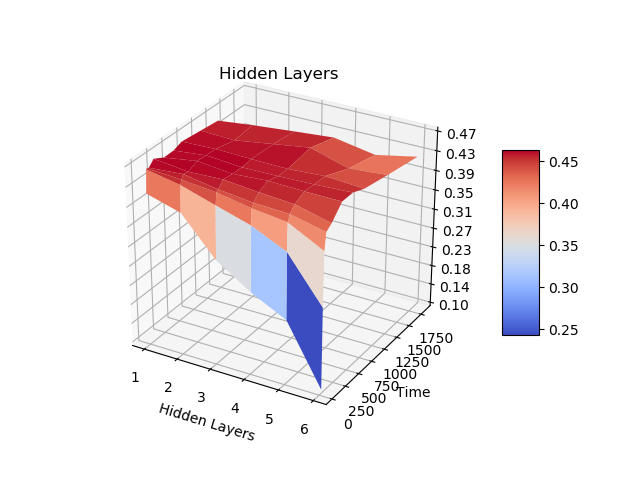
\includegraphics[height=7cm]{pictures/hl_time_fscore.png}
\caption{X: Number of hidden layers, Y: Time, Z: F1-Score}
\label{fig:hl_time_fscore}
\end{figure}

\begin{figure}
     \centering
     \begin{subfigure}[b]{0.3\textwidth}
         \centering
         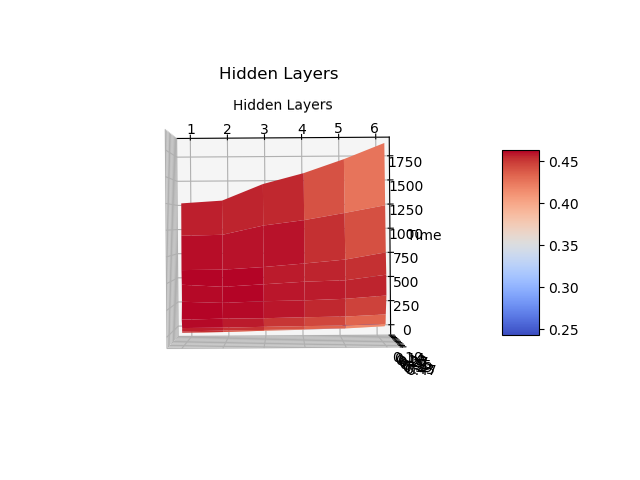
\includegraphics[width=\textwidth]{pictures/hl_time.png}
         \caption{H.l. vs time}
         \label{fig:hl_time}
     \end{subfigure}
     \hfill
     \begin{subfigure}[b]{0.3\textwidth}
         \centering
         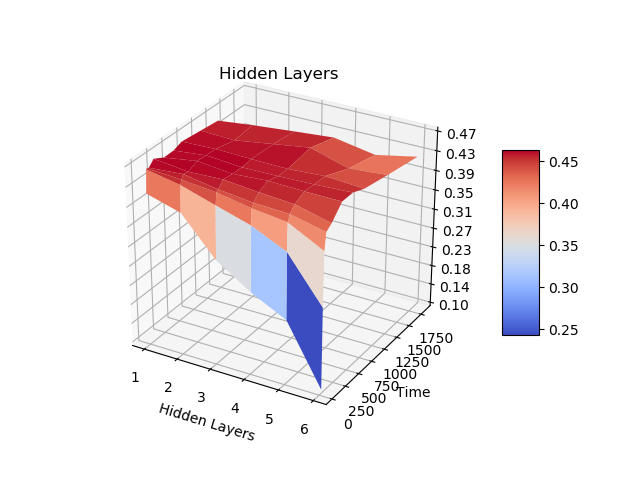
\includegraphics[width=\textwidth]{pictures/hl_time_fscore.png}
         \caption{H.l. vs time vs F1-score}
         \label{fig:hl_time_fscore_small}
     \end{subfigure}
     \hfill
     \begin{subfigure}[b]{0.3\textwidth}
         \centering
         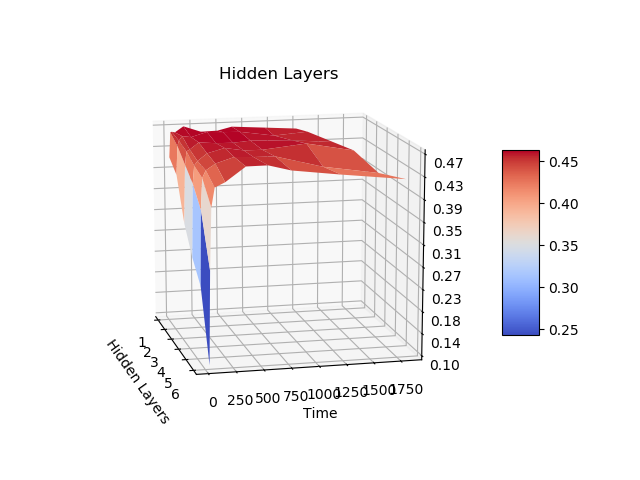
\includegraphics[width=\textwidth]{pictures/hl_time_fscore2.png}
         \caption{H.l. vs time vs F1-score}
         \label{fig:hl_time_score2}
     \end{subfigure}
        \caption{Different views of 3D plot above}
        \label{fig:three3Dgraphs}
\end{figure}

This part of the assignment text specifically asked to analyze how the number of hidden-layers affects computation time. Some subplots showing different views of the 3D plot from Figure \ref{fig:hl_time_fscore} are shown in Figure \ref{fig:three3Dgraphs}.

Specifically, Figure \ref{fig:hl_time} shows the requested relation between hidden-layers and computation times. Here, the different levels on the graph specify the different number of units. This information needs to be implied from looking at the other plots these data generate (when running \href{https://github.uio.no/fabior/IN5550/blob/master/Oblig1/plot.py}{\texttt{plot.py}}). As shown, the general trend of increased computation time is still prevalent as the number of hidden layers increases. The rate of change increases as the number of units per layer grows. This circumstance makes intuitive sense since higher values for both units and hidden-layers directly mean more calculations per epoch.


\subsection{Model evaluations}
\label{chap:Model evaluations}

\subsubsection{Learning rate and momentum}
After finding the optimal \textit{structure} of the neural network, the time had come to evaluate some of the standardized parameters for the model, in hopes to achieve even better model performance. Specifically learning rate and momentum were tuned here. Learning rate was tested with values in the range $\in[0.9, 0.001]$ and momentum in the range $\in[0, 0.9]$. Both of the ranges were chosen to pillow the default values for the respective parameters.

\begin{figure}[H]
\centering
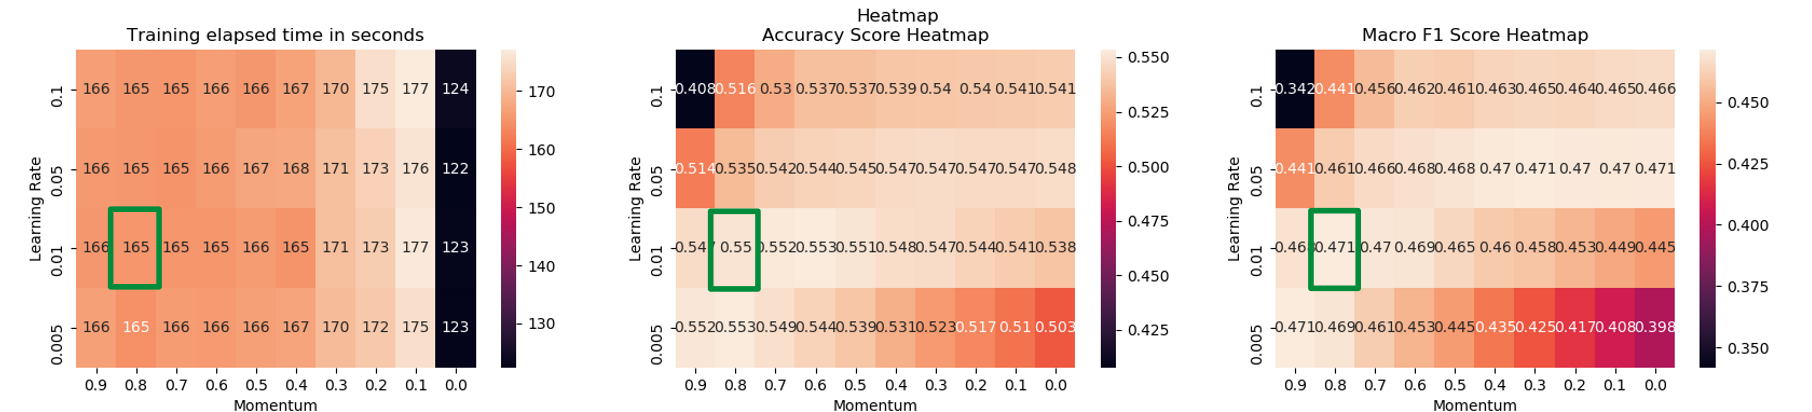
\includegraphics[width=1\linewidth]{pictures/lrm_heatmap.png}
\caption{Learning rate and Momentum heat maps}
\label{fig:lrm_heatmap}
\end{figure}

This evaluation gave no clear winner for either of these parameters, although a trend between their relationship can be observed. It appears that the higher the learning rate is, the lower the momentum needs to be, and vice-versa. To be safe, values within this range that were also close to their defaults were chosen.

And with this step, the tuning of the model was complete and the final hyper-parameters are:

\begin{table}[H]
    \centering
    \begin{tabular}{ |c|c|c|c|c|c| }
        \hline
        \multicolumn{6}{|c|}{\textbf{Hyper-parameters}} \\
        \hline
        \textbf{Hidden Layers} & \textbf{Units} & \textbf{Epoch} & \textbf{Mini-batch} & \textbf{Dropout} & \textbf{Bias} \\
        \hline
        1 & 250 & 5 & 32 & 0.2 & 0.1 \\
        \hline
         \textbf{Learning Rate} & \textbf{Momentum} & \textbf{Loss-Function} & \textbf{HL-Act. Funct.} & \textbf{Out-Act. Funct.} &\\
        \hline
        0.01 & 0.8 & Cross-Entropy & tanh & relu & \\
        \hline
    \end{tabular}
    \caption{Optimized model parameters}
    \label{table:optimal_params}
\end{table}
